\chapter{Theory Introduction}  % should probably change this name
\label{theory}

\section{The Standard Model}
\label{theory:SM}

% quarks, leptons, bosons!  HIGGS ha ha
% make separate paragraphs for different types?  or sections?  that's how other people did it

The Standard Model describes the current understanding 
of how fundamental particles interact.  
There are three different types of particles: 
quarks and leptons, 
which make up matter, 
and bosons, which transmit forces.  
Quarks and leptons are collectively called fermions; 
%because they have spin-$\frac{1}{2}$   % HAVE TO EXPLAIN SPIN AND ALL THAT???
two fermions cannot exist in the same state as each other.  
Bosons do not have this constraint; 
many bosons can be in the same state.  
The particles are shown in Figure~\ref{fig:StandardModel}. 
The first three columns show the first three generations 
of the quarks and leptons, 
while the last column shows the bosons.  
There are six quarks, often represented by their first letters: 
up, down, charm, strange, top, and bottom.  
The first quark in each pair has charge $+\frac{2}{3}$, 
%(in terms of the electron charge), 
while the second has charge $-\frac{1}{3}$.  
These charges are given in terms of the electron charge; 
though the charges are fractional, 
the quarks are always arranged into composite 
particles that have integer multiples of the electron charge.  
The leptons consist of the electron, muon, and tau ($\tau$), 
each with charge -1, 
and their corresponding neutrinos, 
the electron neutrino, muon neutrino, and $\tau$ neutrino, 
which are chargeless.  
Each generation contains two quarks, 
a neutrino, and a charged lepton.  
In general, the generations get progressively heavier.  
The electron is lighter than the muon, 
which is lighter than the $\tau$.   
The same relation exists between the quark generations; 
the top quark is the heaviest particle in the Standard Model.  % CHECK!!!!!
Until recently it was believed that all the neutrinos are massless.  
However, recent experiments indicate 
that neutrinos do have a small mass.  % REFERENCE
Normal, everyday matter is made up solely of particles 
from the first generation.  
All normal matter is made of atoms, 
which in turn consist of a nucleus and 
electrons surrounding the nucleus.  
Atomic nuclei are made of protons and neutrons, 
which are made of up and down quarks: 
the proton by $uud$ and the neutron by $udd$.  
The bosons in the last column transmit the forces 
by which particles interact.  
%The massless photon ($\gamma$) and gluon ($g$) 
%transmit the electromagnetic and the strong forces, 
%respectively, 
The massless photon ($\gamma$) transmits the 
electromagnetic force; this particle is more familiar in its 
everyday context as the particle that makes up light.  
The gluon ($g$), also massless, transmits the strong force, 
which holds protons and neutrons together     %%%%%% STRENGTH OF FORCES, mass of propagator?? but not in all cases
(like glue, hence the name).  
The relatively heavy $Z$ and $W$ bosons 
transmit the weak force, 
which causes nuclear decay.  

%antiparticles
In general, each particle has an antiparticle partner 
of the opposite charge and quantum numbers; % opposite quantum numbers in general, explain quantum numbers? because have to account for photon, gluon, Z, neutrinos
quantum numbers are used to describe the properties of the particles 
and corresponding interactions.  
For instance, all leptons have a non-zero ``lepton number;'' 
if the initial state of a set of particles 
has a total lepton number of 1, 
then any interaction between those particles will 
result in a final state with the same lepton number.  
Lepton number is always conserved in this way, 
as are charge and other quantum numbers.  
The antiparticle of the electron ($e^-$) 
has the opposite charge and lepton number 
and is called the positron ($e^+$).  
Neutrinos, being chargeless, 
have antineutrinos with opposite lepton number.  % EXPLAIN!!!!!
Quarks and gluons have another quantum ``number'' known as color.   % EXPLAIN HOW CANNOT HAVE BARE QUARKS
The three colors are red, green, and blue, with the corresponding 
``anti-colors'' being anti-red, anti-green, and anti-blue.  
%This ``color'' does not refer to our everyday experience of red, green, and blue, 
%%but there is a certain analogy to light in the ``quantum color'' behavior.  
%but the name is not accidental -- there is an analogy to colored light.  
Color is unique in that all observed states of quarks and gluons 
are ``colorless.''
In two-quark states, a color and its anti-color ``combine'' to make a colorless state.  
Three-quark states are also colorless, but through a different combination: 
the three quarks are colored red, green, and blue 
(or the corresponding anticolors), which ``combine'' (like colored light) to form 
a state with no color.
  
Not shown in Figure~\ref{fig:StandardModel} is the Higgs boson, 
which is predicted by the Standard Model 
to give mass to the other particles.  
The Higgs has not yet been discovered; 
finding it (if it exists) is one of the 
goals of the LHC.  

The Standard Model does not include the final 
fundamental force, gravity.  
Gravity is the weakest of the forces and does not 
measurably affect interactions between fundamental particles.  
The reason that it is the only one observable on a 
cosmological scale is because its ``charge,'' mass, 
is cumulative; there is no anti-mass to counter it 
the way a negatively-charge electron and a positively-charged 
proton combine to make an electrically neutral hydrogen atom.  % put this sort of stuff in beginning?
Gravity has been described on a macroscopic scale, but 
%so far gravity has not yet been (fully?) worked into the % FIXME!!!
%framework of the fundamental particles.  
so far no theory has fully united gravity with the 
other fundamental forces.  
%There are many efforts currently ongoing to unite them, % REFERENCE?
%but none of these approaches have yet been proved.  
Such a ``theory of everything'' is a dream of theoretical physics.  

% http://www.symmetrymagazine.org/cms/?pid=1000064  the symmetry magazine SM picture
% don't know how it prints in black and white
% LATEX DOESN'T DO GIFS

 \begin{figure}[htb]
  \begin{center}
%    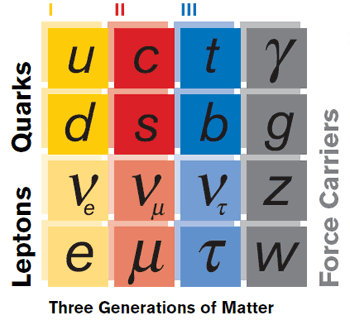
\includegraphics[width=360pt]{Figures/theory-standard-model-symmetry-mag.png}
    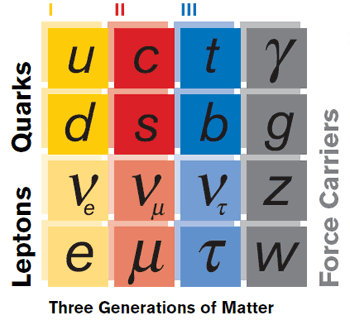
\includegraphics{Figures/theory-standard-model-symmetry-mag.png}
  \end{center}
  \caption[Particles of the standard model]
	  {Particles of the standard model that are known to exist. 
	    The Higgs boson is also predicted as part of the 
	    Standard Model, 
	    but has not yet been discovered. 

	    }
  \label{fig:StandardModel}
 \end{figure}

TABLE OF MASSES



gauge groups, little intro to group theory

A ``group'' is a set of elements with specific properties.  
In particular, any transformation of an element in the group 
results in another element in the group.  

A ``Lie'' group is one in which any transformation 
can be done in very small steps, 
each of which results in an element still in the group.  
The different fundamental forces are described by different Lie groups.  

which particles feel which forces?

Transformations in these groups can be represented as matrices.  
These matrices act on the set of initial states 
and result in the set of final states.  
Each element in the matrix, mapping a single initial state 
to a single other final state, 
gives the amplitude with which the % ONLY IN SCATTERING???  make sure this is right context 
transformation happens.  
Essentially, squaring the matrix element gives the 
relative probability of that particular transformation.  
Matrices are often used to represent transitions 
from one quantum mechanical state to another.  

This is used in particle physics as such: 
a transformation from an initial state, 
in our case two quarks from colliding protons, 
to a final state, 
an electron and a positron, 
is represented by a Feynman diagram, 
shown in Figure~\ref{fig:ZeeFeynmanDiagram}.  
The interaction can be thought to progress to the right.  
Each straight line represents a fermion, 
either the quark or the electron.  
The wavy line represents a boson, the Z.  
(Gluons are represented by curly lines.)  
The intersections between particle lines, or vertices, 
show interactions between the given particles.  
%The type of interaction can be determined by the particles   % NEED THIS?  
%taking part: 
%an interaction between a Z and a quark or lepton 
%indicates the weak force is involved.  
The matrix element corresponding to this transformation 
can be written down 
by attributing factors to the various elements 
of the Feynman diagram, 
the particle lines and the vertices.  

somewhere get into spinors...




put all qcd stuff in here?  don't need all the detail of zeus stuff

\section{Electroweak Physics}
\label{theory:EWK}

lagrangian etc? i.e. more specifics on ewk physics

feynman diagrams, how they can actually be used -> 
matrix elements -> cross section element.  

\begin{figure}[htb]
\begin{center}
  \begin{tikzpicture}[
      thick,
      % Set the overall layout of the tree
%      level/.style={level distance=1.4cm, line width=0.8mm},
      level/.style={level distance=1.4cm, line width=0.5mm},
      level 2/.style={sibling distance=1.4cm},
      level 3/.style={sibling distance=1.4cm}
    ]
    \coordinate
%    child[grow=south east]{
%      child[grow=north east]{
%        edge from parent [gluon]
%        node[right]{$g$}
%      }
    child[grow=south east]{
      edge from parent [electron]
      child[grow=south west] {
        edge from parent [electron]
%        node[above] {$\bar{q}$} % ADDED
        node[below] {$\bar{q}$} % ADDED
%          child[grow=south west]{
%            edge from parent [electron]
%            node[above] {$\bar{q}$}
%          }
%          child[grow=south east]{
%            edge from parent [gluon]
%            node[right] {$g$}
%          }
      }
      child[grow=east, level distance=2.4cm] {
        child[]{ % added the [], did nothing, don't know how to make angle of line the same as LHS
          edge from parent [electron]
          node[below] {$e^{-}$}
        }
        child[]{ % added the [], did nothing, don't know how to make angle of line the same as LHS
          edge from parent [electron]
          node[above] {$e^{+}$}
        }
        edge from parent [boson]
%        node[below] {$Z/\gamma*$}
        node[below] {$Z$}
      }
%    }
      edge from parent [electron] node [above=3pt] {$q$}
    };
  \end{tikzpicture}
\end{center}
%  \caption[Feynman diagram of \qqZgee]
  \caption[Feynman diagram of \qqZee]
%	  {Feynman diagram of \qqZgee.  
	  {Feynman diagram of \qqZee.  
	    }
  \label{fig:ZeeFeynmanDiagram}
\end{figure}

where to put cross section formula stuff 
-- make new section?
(and which stuff to use?)

order of diagram = number of vertices!  

\subsection{Z Production}
\label{theory:Zprod}

previous results here?

\subsection{Z Decay}
\label{theory:Zdec}
need this section??


somewhere have intro to QFT and all that?  

also, explanatory items from overview:

   * [here or] in theory chapter define ``tree-level''.  
ALSO IN THEORY: explain how Feynman diagrams are so useful! 
writing down the matrix element and all that
AND PDFs, basically whole process of stuff simulated 
really happens and should be explained.  
AND DEF OF PARTONS
yeah, basically explain all the stuff in the MC chapter
INCLUDING ISR and FSR
ALSO define ``jets'' and talk about how they come from 
quarks and gluons (define partons) and relate to ``hadronization'' -- 
not entirely relevant for this analysis, 
but possible in general
AND define ``color''
AND asymptotic freedom, how it takes more and more energy to get them further apart

   * intial- and final-state radiation

   * [HERE OR IN THEORY INTRO] need to do on-shell/off-shell decays 
to explain why Z mass has a spectrum and not a single value

   * invariant mass (here?)

   * cross section formula and matrix elements and what said matrices do

AND, of course read the others' theses to see what they had in here, too.  



